% This is LLNCS.DEM the demonstration file of
% the LaTeX macro package from Springer-Verlag
% for Lecture Notes in Computer Science,
% version 2.4 for LaTeX2e as of 16. April 2010
%
\documentclass{llncs}
%
%\usepackage{makeidx}  % allows for indexgeneration
\usepackage{ragged2e}
\usepackage{parskip}
\usepackage{wrapfig}
\usepackage{array}
\usepackage{float}
\usepackage[english]{babel}
\usepackage{lipsum}
\usepackage{caption}
\usepackage{subcaption}
\usepackage{graphicx}
\graphicspath{{images/}} 
\usepackage[linesnumbered,ruled]{algorithm2e}
\usepackage{courier}
\usepackage{hyperref}
\hypersetup{colorlinks=true,allcolors=blue}
\usepackage{listings}
\lstset{
    basicstyle=\ttfamily,
    frame=none, 
    breaklines=true,
    numbers=left,
    xleftmargin=2.5em,
    framexleftmargin=0em,
    emphstyle=\textbf,
    float=t
}
\lstdefinestyle{ocl}{
    emph={
context, inv
    }
}
\lstdefinestyle{cbp}{
    basicstyle=\ttfamily\scriptsize,
    emph={
session, create, of, type,
set, to, add, hire
    }
}
\lstdefinestyle{xmi}{
    basicstyle=\ttfamily\scriptsize,
    emph={
Node, children
    }
}
\lstdefinestyle{xml}{
    basicstyle=\ttfamily\scriptsize,
    emph={
register, create, add, to, resource,
from, eattribute, remove, ereference,
set, unset, session, Roy, Jen,
Moss, Richmond
    }
}
\lstdefinestyle{java}{
    basicstyle=\ttfamily\scriptsize,
    emph={
case, $unset$,
instanceof, else, if, void,
new, UnsetEAttributeEvent,
UnsetEReferenceEvent,
@override, public, class, extends
    }
}
\lstdefinestyle{eol}{
    basicstyle=\ttfamily\scriptsize,
    emph={
var, new, for, in, create, set, of, with, 
unset, to, add, remove, delete, register, move,
from, position, from, move-within, session, \.
    }
}

\begin{document}
    \renewcommand{\thelstlisting}{\arabic{lstlisting}}
    \renewcommand{\labelitemi}{$\bullet$}
    \newcommand{\dk}[1]{\textbf{[DK: #1]}}
    
    \title{Towards Efficient Loading \\ of Change-Based Models}
    %
    \titlerunning{Towards Efficient Loading of Change-Based Models}  % abbreviated title (for running head)
    %     also used for the TOC unless
    %     \toctitle is used
    %
    \author{
Alfa Yohannis \and Horacio Hoyos Rodriguez \and Fiona Polack$^*$ \and Dimitris Kolovos
    }
    %
    \authorrunning{
Alfa Yohannis et al.
    } % abbreviated author list (for running head)
    %
    %%%% list of authors for the TOC (use if author list has to be modified)
    %\tocauthor{Alfa Yohannis,Horacio Hoyos Rodriguez, Fiona Polack, Dimitris Kolovos}
    %
    
    \institute{anonym}
    \institute{Department of Computer Science, University of York, United Kingdom\\$^*$School of Computing and Maths, Keele University, United Kingdom\\
    \email{\{ary506, horacio.hoyos, dimitris.kolovos\}@york.ac.uk\\$^*$f.a.c.polack@keele.a.cuk}}
    
    \maketitle      % typeset the title of the contribution
    %The first states the problem. The second states why the problem is a problem. The third is my startling sentence. The fourth states the implication of my startling sentence.
    \begin{abstract}
This paper proposes and evaluates an efficient approach for loading models stored in a change-based format. The work builds on language-independent change-based persistence (CBP) of models conforming to object-oriented metamodelling architectures such as MOF and EMF, an approach which persists a model's editing history rather than its current state. We evaluate the performance of the proposed loading approach and assess its impact on saving change-based models. Our results show that the proposed approach significantly improves loading times compared to the baseline CBP loading approach, and has a negligible impact on saving.

    \end{abstract}
    
    \section{Introduction}
    \label{sec:introduction}
    Conventional approaches for file-based model persistence in metamodelling architectures such as MOF \cite{omg2018mof} and EMF \cite{steinberg2008emf} are state-based -- saving the current state of a model.  In these approaches,  version control and change detection are delegated to external systems.  State based persistence is computationally expensive, as a whole model must be saved and loaded; this particularly effects large models and collaborative developments.
    
    In \cite{yohannis2017turning}, we proposed change-based persistence (CBP), an approach that persists the full sequence of \emph{changes} made to a model instead of persisting the state. Compared to state-based approaches, CBP supports fast detection of changes, which can speed up model comparison and merging, as well as fast incremental model validation and transformation \cite{rath2012derived,ogunyomi2015property}. However, saving the change history of a model results in large, and ever-growing, CBP files.  Loading times are also significant, as the loading process has to reconstruct a model's current state from its history \cite{yohannis2017turning}.   This paper proposes and evaluates an approach that reduces CBP model loading time by avoiding the replaying of historical changes that have no impact on the final state of the model.
    
    The rest of the paper is structured as follows. Section \ref{sec:case_study} introduces a running example and provides a brief introduction to CBP.
    Section \ref{sec:loading_time_optimisation} presents the approach to speed up model loading and its supporting data structures. Section \ref{sec:performance_evaluation} presents experimental results and evaluation. Section \ref{sec:related_work} provides an overview of related work, and Section \ref{sec:conclusions} concludes with discussion of directions for future work.
    
    \vspace{-15pt}
    \section{Running Example}
    \label{sec:case_study}
    \vspace{-10pt}
    To explain model CBP, we use a minimal tree metamodel and an example tree model in Figures \ref{fig:tree_metamodel} and \ref{fig:initial_model}.
    The metamodel is expressed the Eclipse Modelling Framework (EMF) Ecore metamodelling language, the de-facto standard for object-oriented metamodelling.  The example is contrived to avoid unnecessary repetition, whilst providing adequate coverage of the core features of Ecore (classes, single/multi-valued features, references).
    In this example, a tree model consists of named nodes which can -- optionally -- contain other nodes ($child$ reference).
    
    \vspace{-20pt}
    \begin{figure}[ht]
        \begin{subfigure}[t]{0.3\linewidth}
            \centering
            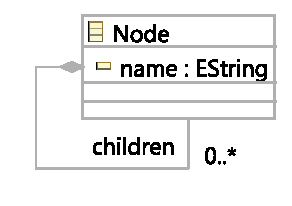
\includegraphics[width=0.8\linewidth]{node_metamodel}
            \caption{The tree metamodel (EMF/Ecore).}
            \label{fig:tree_metamodel}
        \end{subfigure}
        \hfill
        \begin{subfigure}[t]{0.7\linewidth}
            \centering
            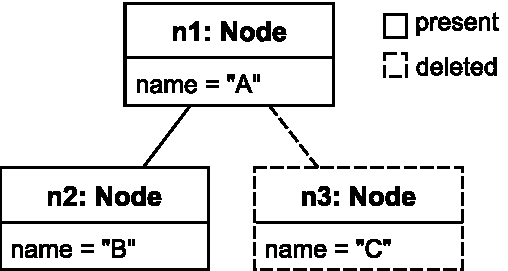
\includegraphics[width=0.6\linewidth]{initial_chart}
            \caption{A tree model that conforms to the  metamodel.  Node n3 is created and then deleted.}
            \label{fig:initial_model}
        \end{subfigure}
        \caption{Running example of a metamodel and a conformant model.}
        \label{fig:append_speed}
    \end{figure}

\vspace{-10pt}
    The current state of the model in Figure \ref{fig:initial_model} has two nodes, $n1$, $n2$.  The model was constructed by firstly creating the three nodes ($n1$, $n2$ and $n3$) and then nodes $n2$ and $n3$ were then added as children of $n1$. Finally, node $n3$ was deleted.
    
    \vspace{-10pt}
\begin{minipage}[t]{0.5\linewidth}
\begin{lstlisting}[style=xmi,caption={State-based tree model.},label=lst:xmimodel]
<Node id="n1" name="A">
<children id="n2" name="B"/>
</Node>
\end{lstlisting}
\end{minipage}
\hfill
\begin{minipage}[t]{0.5\linewidth}
\begin{lstlisting}[style=eol,caption={Change-based tree model.},label=lst:cbpmodel]
create n1 of Node
set n1.name to "A"  
create n2 of Node
set n2.name to "B"  
create n3 of Node
set n3.name to "C"  
add n2 to n1.children   
add n3 to n1.children
remove n3 from n1.children   
delete n3
\end{lstlisting}
\end{minipage}

    Listings \ref{lst:xmimodel} shows the state-based representation of the model, using simplified XMI.  Listing \ref{lst:cbpmodel} shows the change-based representation, using the CBP syntax introduced in \cite{yohannis2017turning}. Lines 1-6 of Listing \ref{lst:cbpmodel} record the creation and naming of the three nodes; lines 7-8 record the addition of $n2$ and $n3$ as children of $n1$; lines 9-10 capture the deletion of $n3$ (the $remove$ command removes f $n3$ from its container; the $delete$ command completely removes $n3$ from its model). Changes in a CBP representation can be uniquely identified by their line numbers.
    
    The example model history illustrates a case where  earlier events (creating \emph{n3} in line 5, naming it in line 6, making it a child of \emph{n1} in line 8, removing it from the container in line 9) are superseded by a subsequent event (deletion of \emph{n3} in line 10).  Loading of the current model would arguably be faster if the events in lines 5, 6, 8, 9 and 10 could be ignored.
    
    \vspace{-10pt}
    \section{Towards Efficient Loading of Change-Based Models}
    \label{sec:loading_time_optimisation}
    
    \vspace{-10pt}
    The flowchart in Figure \ref{fig:flowchart} provides an overview of the editing lifecycle of a CBP model \cite{yohannis2017turning}, with the proposed extensions shown as starred blocks. A model is loaded (1), edited (2) and saved (3).  During editing, the changes made to the model are recorded in a memory-based data structure, serialised and with the latest event appended at the end (4). The change events are persisted into a CBP file every time the model is saved (5). When a model is re-loaded, the current model state is recreated from the saved CBP file (6).
    
    \vspace{-10pt}
    \begin{figure}[ht]
        \centering
        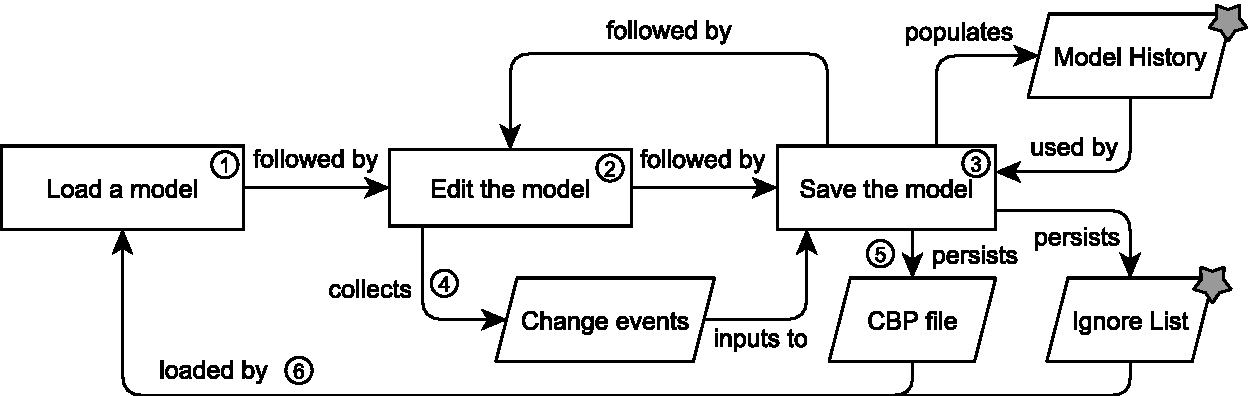
\includegraphics[width=\linewidth]{flowchart}
        \caption{CBP workflow, with optimised loading elements indicated by starred blocks.}
        \label{fig:flowchart}
    \end{figure}

    \vspace{-10pt}
    A key principle of CBP is that the editing history is immutable, as this is essential for supporting incremental model management operations. As such, superseded events cannot be simply removed from the CBP file. Therefore, the proposed approach adds two artefacts: a $Model History$ data structure which aggregates change events per model element, and an $Ignore List$ file, which persists the position (i.e. line numbers) of superseded events so that the events can be ignored the next time the model is loaded. The Ignore List is saved alongside the CBP file. The rest of this section presents how the Model History is used to detect superseded events and generate the Ignore List.
    
    \vspace{-10pt}
    \subsection{Model History}
    \label{subsec:model_history}
    The Model History data structure stores events and their line numbers in a CBP representation.  The data can be used to reason about the events of a particular element and to determine which events are superseded.  We refer to the line number in the CBP representation as the \emph{event number}. The proposed data structure is defined in Figure \ref{fig:object_history} using a class diagram.  
     
    A \emph{ModelHistory} has a \emph{URI} attribute to identify the model for which it records changes.  A \emph{ModelHistory} can link to many \emph{ElementHistory} objects, each identified by its \emph{element} field which is queried from the model. An \emph{ElementHistory} can link to many \emph{FeatureHistories}, representing the editing histories of individual features -- either references or attributes of the element. A \emph{FeatureHistory} has a \emph{type} (attribute or reference) and a \emph{name}, identifying the feature.

\vspace{-20pt}    
\begin{figure}[ht]
\centering
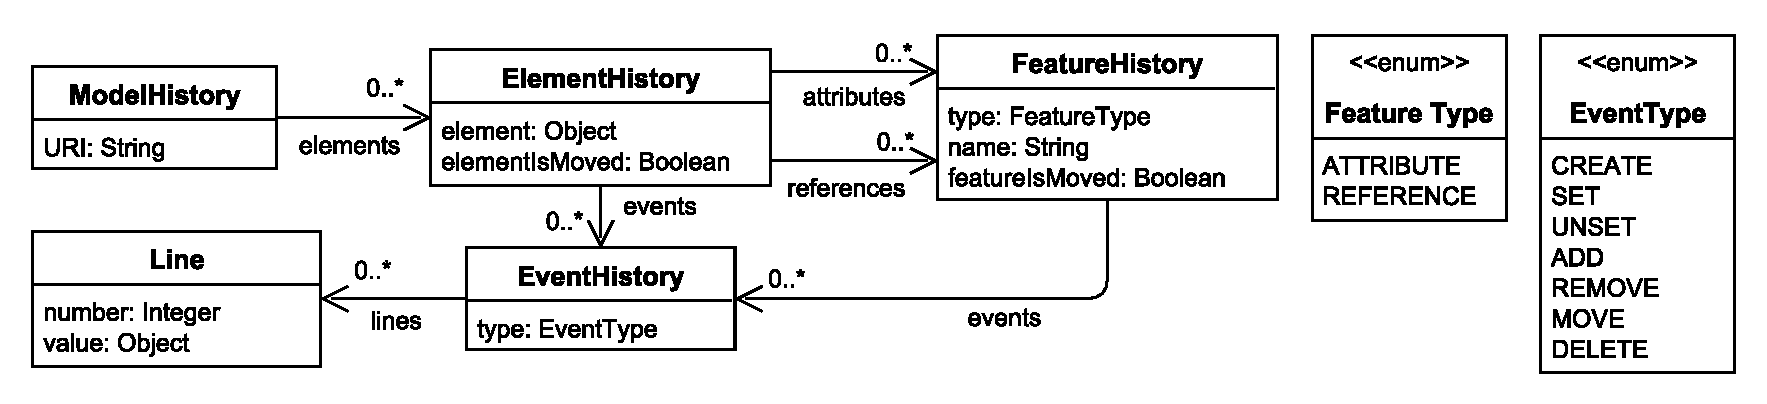
\includegraphics[width=\linewidth]{object_history}
\caption{The class model defining Model History.}
\label{fig:object_history}
    \end{figure}

\vspace{-30pt}
\begin{figure}[ht]
\centering
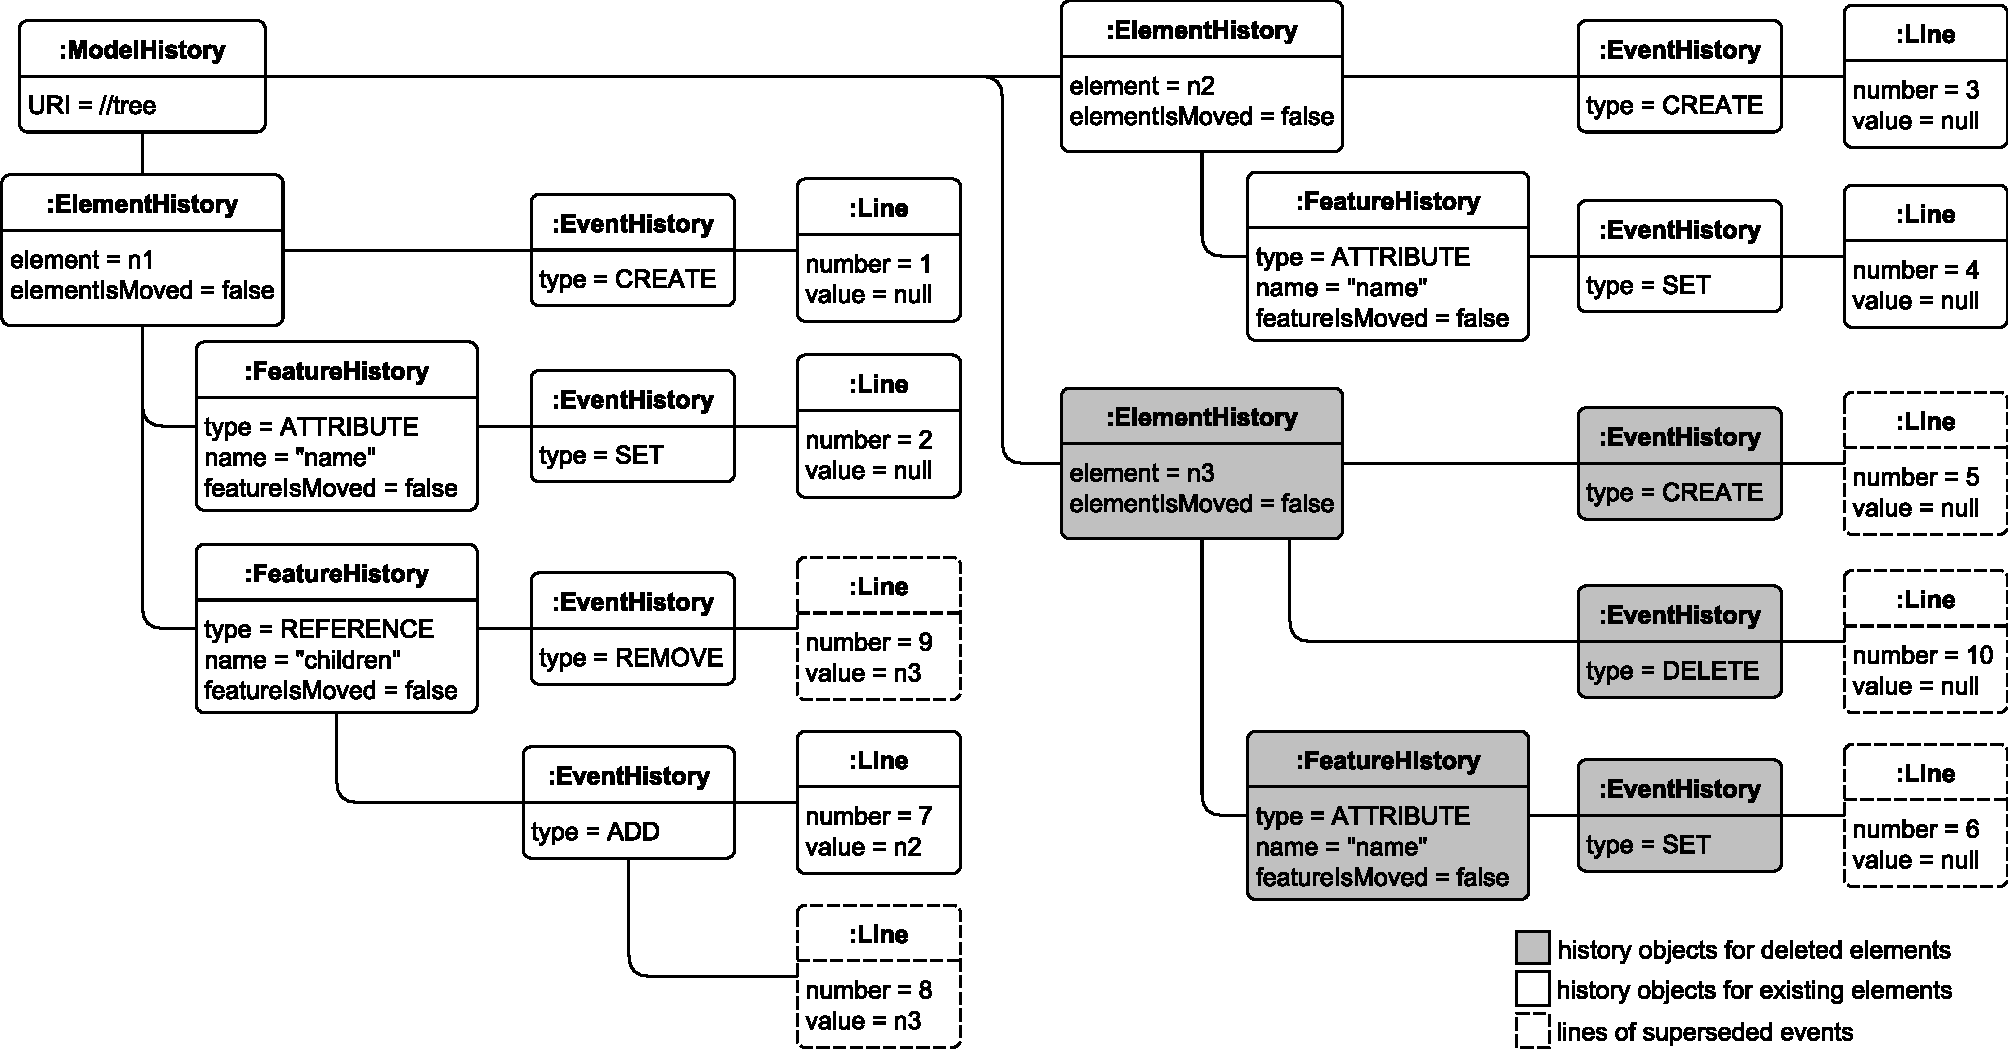
\includegraphics[width=\linewidth]{history_structure}
\caption{The object diagram of the CBP model history in Listing \ref{lst:cbpmodel}.}
\label{fig:history_structure}
\end{figure}
    
    
    An \emph{EventHistory} represents series of events of the same type; it has an attribute \emph{type} to identify the events' type, and can have many \emph{Line}s. A \emph{Line} has a \emph{number} attribute, to record the event number, and a \emph{value} that records the element involved in the event (Value is only used for events with types \emph{$ADD$}, \emph{$REMOVE$} and \emph{$MOVE$}). Each \emph{FeatureHistory} can have many \emph{EventHistories}, to represent the events that modify the values of the features. Each \emph{ElementHistory} can have many \emph{EventHistories} to represent events that affect the state of the elements (life-cycle and relations to multivalued features). Figure \ref{fig:history_structure} shows an object diagram corresponding to the model in Figure \ref{fig:object_history} that captures the model history shown in Listing \ref{lst:cbpmodel}. The grey rectangles are \emph{History} objects related to the deleted node \emph{n3}. The rectangles with the dashed outline are \emph{Line} objects that represent superseded changes. 
    
    Next, we present the different strategies used to identify superseded events that will be added to the Ignore List.   
    
    \vspace{-10pt}
    \subsection{Set and Unset Events}
    \label{subsec:set_and_unset_operations}
    During the lifecycle of a model, a single-valued feature can have a value set (assigned) or unset many times. Each event is persisted, but only the last assigned value needs to be considered. For example, in Listing \ref{lst:set_unset_example_1}, the feature \emph{name} is set to the value ``A'', unset, and finally set to the value ``B''.  In the final state of the model, \emph{n1.name} = ``B''. Thus, only line 4 that is significant for the model's final state and therefore lines 2 and 3 can be ignored when loading the model. A specific rule applies to an $unset$ event. It can be ignored along with all preceding $set$ and $unset$ events. Executing it does have any affect to final state of a model if all the preceding events also have been ignored -- not executed.
    
    \vspace{-10pt}
    \begin{minipage}[t]{0.49\linewidth}
\begin{lstlisting}[style=eol,caption={A CBP representation of attribute \emph{name} assignments.},label=lst:set_unset_example_1]
create n1 of Node
set n1.name to "A"
unset n1.name
set n1.name to "B"
\end{lstlisting}
    \end{minipage}
    \hfill
    \begin{minipage}[t]{0.49\linewidth}
\begin{lstlisting}[style=eol,caption={A CBP representation of attribute \emph{name} assignments.},label=lst:set_unset_example_2]
create n1 of Node
set n1.name to "A"
set n1.name to "B"
unset n1.name
\end{lstlisting}
    \end{minipage}
    
    Based on the Listing \ref{lst:set_unset_example_1}, our approach creates an instance of $ElementHistory$ $n1$ which contains an instance of $FeatureHistory$ $name$. The $FeatureHistory$ $name$ consists of two $EventHistory$ instances, with types $SET$ and $UNSET$ (the instances are named $set$ and $unset$ respectively for brevity). The $set$ records the $Line$ instances that hold the the event numbers where the $set$ events, and similarly for $unset$.
    
    From Listing \ref{lst:set_unset_example_1}, we can thus infer that $name$.$set$.$lines$ = $\{2,4\}$ and $name$.$unset$. $lines$ = $\{3\}$. The event numbers in both lists are used to determine that the events represented by lines 2 and 3 are superseded by that in line 4, which is a $set$ event, giving an $ignoreList$ = $\{2, 3\}$.  By the same process, for Listing \ref{lst:set_unset_example_2}, we can reason that $name$.$set$.$lines$ = \{2,3\} and $name$.$unset$.$lines$ = \{4\}.  However, this case, the highest-numbered event is an $unset$, all so line numbers are put into the $ignoreList$ ($ignoreList$ = $\{2, 3, 4\}$) ($unset$ event can be ignored along with all preceding {$set$ and $unset$ events). 
    
    \vspace{-10pt}
    \subsection{Add, Remove, and Move Events}\label{subsec:add_remove_and_move_operations}
    For a multi-valued feature, events add, remove and move can be called many times, to modify the feature. If an element is added to the feature, moved multiple times, and finally removed, then all the element's preceding events can be ignored, as long as the order of the feature's elements is not changed. 
    

    
    Listing \ref{lst:add_move_reference} shows an example without a $move$ event. In the Listing, nodes $n1$, $n2$, and $n3$ are added to the $children$ feature of $p$ (lines 5-7), In the latest state of the model, $children$ only contains $n1$ and $n3$. As a result, the loading process could ignore the events that represent the \textit{$add$} and \textit{$remove$} events on $n1$. 
    
    \vspace{-20pt}
    \begin{minipage}[t]{0.34\linewidth}
\begin{lstlisting}[style=eol,caption={A CBP of add and remove operations.},label=lst:add_move_reference]
create p of Node
create n1 of Node
create n2 of Node
create n3 of Node
add n1 to p.children
add n2 to p.children
add n3 to p.children
remove n2 from p.children   
\end{lstlisting}
    \end{minipage}
    \hfill
    \begin{minipage}[t]{0.62\linewidth}
\begin{lstlisting}[style=eol,caption={A CBP representation of add, move, and remove operations.},label=lst:add_remove_move_reference]
create p of Node          //children=[]
create n1 of Node         //children=[]
create n2 of Node         //children=[]
create n3 of Node         //children=[]
add n1 to p.children      //children=[n1]
add n2 to p.children      //children=[n1,n2]
add n3 to p.children      //children=[n1,n2,n3]
move 0 to 1 in p.children //children=[n2,n1,n3]
remove n2 from p.children //children=[n1,n3]
\end{lstlisting}
    \end{minipage}

    To create the Ignore List for the Listing \ref{lst:add_move_reference}, we can deduce that $children$.$add$. $lines$ = \{\{5, $n1$\}, \{6, $n2$\} \{7, $n3$\}\} (5 is the line number and $n1$ is the value) and $children$.$remove$.$lines$ = \{\{8, $n1$\}\}. Since $n2$ is removed from its containing feature (line 8), then executing its preceding add and remove events is unnecessary. Note that we retain the $create$ event (line 3) as $n2$ has not been deleted from the model -- only removed from its containing feature. We can iterate through the add and move structures to identify the events on $n2$ that should be removed, resulting in the $ignoreList$ = \{6, 8\}.
    
    Listing \ref{lst:add_remove_move_reference} shows an example with a $move$ event. A $move$ event is inserted at line 8 shifted the $remove$ event of $n2$ to line 9. With the introduction of this $move$ event, we now have the $children$.$add$.$lines$ = \{\{5, $n1$\}, \{6, $n2$\} \{7, $n3$\}\}, $children$.$move$.$lines$ = \{\{8, $n1$\}\}, and $children$.$remove$.$lines$ = \{\{9, $n2$\}\}. In the final state of the model, the $children$ should have the $n1$ and $n3$ in order, $children$ = [n1, n3] (The commented parts of Listing \ref{lst:add_remove_move_reference} show the end states of $children$ after each event).  
    
    However, executing the previous strategy naively leads to an error final state. Using $ignoreList$ = \{6, 8\} produced by the naive strategy leads to different order of $n1$ and $n3$ in the final state of the model where $children$ = [n3, n1] as shown by the naive optimised CBP in Listing \ref{lst:naive_add_remove_move_reference}. To prevent this problem, *$IsMoved$ flags in Figure\ref{fig:object_history} is used to sign  features and elements if they have been moved -- the flags are set to $true$. If an element's *$IsMoved$ flag is true then all of its line numbers related to $add$, $move$, $remove$ events cannot be put into the $ignoreList$. The flags is set to $false$ if the feature is empty. 

\begin{lstlisting}[style=eol,caption={A naive optimised CBP representation of original CBP representation in Listing \ref{lst:add_remove_move_reference} .},label=lst:naive_add_remove_move_reference]
create p of Node            // children = []
create n1 of Node           // children = []
create n2 of Node           // children = []
create n3 of Node           // children = []
add n1 to p.children        // children = [n1]
add n3 to p.children        // children = [n1, n3]
move 0 to 1 in p.children   // children = [n3, n1]
\end{lstlisting}

    \subsection{Create and Delete Events}
    \label{subsec:create_and_delete_operations}
    
    When an element is deleted, it is completely removed from the model. Therefore, all previous events ($create$, $set$, $unset$, $move$, $add$, $remove$, $delete$) on that element can be ignored, along with all events on the element's features. For example, when node \emph{n3} in Listing \ref{lst:cbpmodel} is deleted, the events in lines 5-6 and 8-10 are superseded. The optimised change-based representation of Listing \ref{lst:cbpmodel} is presented in Listing \ref{lst:cbpmodel_optimised}.
    
    \begin{lstlisting}[style=eol,caption={Change-based representation of the model in Figure \ref{fig:initial_model} after removal of node \emph{n3}.},label=lst:cbpmodel_optimised]
create n1 of Node
set n1.name to "A"
create n2 of Node
set n2.name to "B"
add n2 to n1.children
    \end{lstlisting}
    
    Using the Listing \ref{lst:cbpmodel}, we can construct the structure of histories that are related to element $n3$ as follows: $n3$.$create$.$lines$ = \{5\}, $n3$.$name$.$set$.$lines$ = \{6\}, $n1$.$children$.$add$.$lines$ = \{\{7, $n2$\}, \{8, $n3$\}\}, $n1$.$children$.$remove$.$lines$ = \{\{9, $n3$\}\}, and $n3$.$delete$.$lines$ = \{10\}. Thus, when element $n3$ is deleted, by iterating through all these history structures, all line numbers associated with $n3$ can be identified and added to $ignoreList$ producing $ignoreList$ = \{5 6, 8, 9, 10\} so they can be ignored in the next model loading.
    
    \section{Performance Evaluation}
    \label{sec:performance_evaluation}
    
    We developed the proposed efficient loading approach on top of the original CBP implementation\footnote{The prototype, tests, and data used in the evaluation are available under \url{https://github.com/epsilonlabs/emf-cbp} and \url{https://goo.gl/1zUBQC} for reproducibility} from \cite{yohannis2017turning} and evaluated our approach's model loading performance, as well as its memory footprint and its impact on the time required to save changes made to CBP models. The evaluation was performed on Intel\textsuperscript{\textregistered} Core\textsuperscript{TM} i7-6500U CPU@2.50GHz 2.59GHz, 12GB RAM, and the Java\textsuperscript{TM} SE Runtime Environment (build 1.8.0\textunderscore162-b12).
    
    Given that CBP is a very recent contribution and we are not aware of any existing datasets containing real-world models expressed in a change-based format, we have used synthetic change-based models for the evaluation of our experiments. The synthetic models were derived from real-world cases: the BPMN2 \cite{eclipse2017bpmn2,eclipse2018bpmn2git} and Epsilon \cite{eclipse2017epsilon,eclipse2018epsilongit} software projects, and the article on the United States \cite{wikipedia2018us} on Wikipedia. For the first two projects, for each version of the cases, we used MoDisco \cite{DBLP:journals/infsof/BruneliereCDM14} to generate a UML2 \cite{eclipse2017uml2} model that reflects its source code. For the Wikipedia article, a model that conforms to the Modisco XML metamodel \cite{eclipse2018modiscoxml} was generated. Since these cases have many versions -- represented by commits/revisions, different models of the versions can be generated and to some degree they reflect the time-ordered changes of the cases. The synthetic change-based model for each case was derived by comparing an initially-empty running model to different versions of the case's models sequentially. All identified differences were then reconciled by performing a unidirectional merging to the running model. All changes made to the running model during the merging process were captured and persisted into a CBP file. EMF Compare was used \cite{eclipse2017compare} to perform the comparison and merging.
    
    Using the synthetic models, we performed performance evaluation on loading time, saving time, and memory footprints for both loading and saving. To compare the loading time, we ran the optimised and original (baseline) CBP algorithms to reconstruct the current state of each of the three models (The results are shown in Figure \ref{fig:loadtime}). As discussed in Section \ref{sec:loading_time_optimisation}, optimised CBP also does extra work when saving the changes to a model, in order to save time (relative to original CBP) when loading a model. To analyse the perfomance effect of optimisation activities, we therefore compared the overall time required to save a new version of the models described above, after one single change has been made (The results are shown in Figure \ref{fig:savetime}). we also compare the memory footprints for both loading and saving since the optimised CBP approach also requires the maintenance of an additional in-memory data structure that keeps track of element and feature editing histories (See Figure \ref{fig:loadmemory} and \ref{fig:savememory} for the results). 
    
    For each combination of dimensions (loading time, saving time, loading memory footprint, saving memory footprint),  persistence types (original CBP, optimised CBP, and XMI), and cases (BPMN2, Epsilon, and United States), we performed measurement 22 times. The results of the measurement enabled us to perform the Welch's t-test \cite{welch1947ttest} to find the significance of the comparisons for each case. For loading and saving time, we measured the delta time required to complete the loading and saving. For memory footprint, we measured the delta of memory used before and after loading and saving completes. We also collected some data description to characterise our cases. The results are presented in the following subsections.

\subsection{Data Description}
\label{subsec:data_description}

\vspace{-25pt}
\begin{table} [ht]
    \centering
    \caption{Description of change-based models generated for evaluation.}
    \label{table:data_description}
    \begin{tabular}{|>{\centering\arraybackslash}p{1.5cm}|>{\centering\arraybackslash}p{1.7cm}|>{\centering\arraybackslash}p{2.4cm}|>{\centering\arraybackslash}p{1.6cm}
            |>{\centering\arraybackslash}p{1.5cm}|>{\centering\arraybackslash}p{2cm}|}
        \hline 
        \textbf{Model} & \textbf{Total Events} & \textbf{Ignored Events} & \textbf{Elements} & \textbf{Total Versions} & \textbf{Processed Versions} \\
        \hline
        BPMN2 & \multicolumn{1}{r|}{1,238,752} & \multicolumn{1}{r|}{1,078,058 (87.0\%)} & \multicolumn{1}{r|}{62,062} & \multicolumn{1}{r|}{192} & \multicolumn{1}{r|}{192 (100.0\%)} \\
        \hline
        Epsilon & \multicolumn{1}{r|}{2,593,044} & \multicolumn{1}{r|}{1,775,895 (68.5\%)} & \multicolumn{1}{r|}{79,459} & \multicolumn{1}{r|}{3,037} & \multicolumn{1}{r|}{727 (23.9\%)} \\
        \hline 
        Wikipedia & \multicolumn{1}{r|}{11,488,143} & \multicolumn{1}{r|}{7,765,000  (67.6\%)} & \multicolumn{1}{r|}{12,144} & \multicolumn{1}{r|}{37,996} & \multicolumn{1}{r|}{3,100 (8.2\%)} \\
        \hline 
    \end{tabular}
\end{table}

Table \ref{table:data_description} summarises events, elements and saved versions for the Epsilon, BPMN2, and Wikipedia cases. Total Events is the numbers of events that were produced by our approach in generating a change-based model for each case.  Ignored events is the number of superseded events that do not need to be replayed when reloading the models. Elements is the number of elements contained in each model. Total versions is the number of commits/revisions made to the cases, taken from the git repositories or Wikipedia at the time this evaluation performed. Processed versions is the number of commits/revisions that were processed to produce change-based models: since the comparison between versions takes considerable time, not all versions are processed here.

\subsection{Model Loading Time}
\label{subsec:loading_time_test}

 This subsection presents the results of the loading time measurement of change-based models for each pair of the persistence types and cases and the t-test results of their comparisons (Table \ref{table:ttest_results_loadtime} and Figure \ref{fig:loadtime}). 
 
 \vspace{-10pt}
 \begin{table}[ht]
     \footnotesize
     \centering
     \caption{The t-test results of loading time comparison between original CBP (CBP), optimised CBP (OCBP), and XMI.}
     \label{table:ttest_results_loadtime}
     \begin{tabular}
         {|p{0.09\textwidth}|p{0.16\textwidth}|p{0.16\textwidth}|p{0.21\textwidth}|p{0.10\textwidth}|p{0.10\textwidth}|p{0.12\textwidth}|}
         \hline 
         
         % BPMN2 Load Time
         \textbf{Group} & \textbf{Mean} & \textbf{SD} & \textbf{Comparison} & \textbf{t}  & \textbf{df} & \textbf{p-value} \\  
         \hline 
         \multicolumn{7}{|c|}{BPMN2 Load Time} \\
         \hline 
         \textbf{CBP} & 5.8119463   & 0.078829340 & \textbf{CBP vs XM}I & 315.95    &21.462 & $<$ 2.2e-16 \\  
         \hline 
         \textbf{OCBP} & 3.0187454   & 0.126962479 & \textbf{CBP vs OCBP} & 87.667 & 35.096  & $<$ 2.2e-16 \\  
         \hline 
         \textbf{XMI} &0.4727595   & 0.4727595 & \textbf{OCBP vs XMI} & 93.858    & 21.178  & $<$ 2.2e-16 \\ 
         \hline 
         
         % EPSILON Load Time
         \multicolumn{7}{|c|}{Epsilon Load Time} \\
         \hline 
         \textbf{CBP} & 16.6016844    & 0.22671101 &  \textbf{CBP vs XM}I & 324.18   &22.782 & $<$ 2.2e-16 \\
         \hline 
         \textbf{OCBP} &  8.2764839  &  0.09011991 & \textbf{CBP vs OCBP} & 160.06 & 27.475 & $<$ 2.2e-16 \\  
         \hline 
         \textbf{XMI} & 31.537   & 0.04674494 & \textbf{OCBP vs XMI} & 354.52   &42.055  & $<$ 2.2e-16 \\ 
         \hline 
         
         % WIKIPEDIA Load Time
         \multicolumn{7}{|c|}{United States Load Time} \\
         \hline 
         \textbf{CBP} & 34.23280361     & 0.1445454700 & \textbf{CBP vs XM}I & 1110.1   &21.001 & $<$ 2.2e-16 \\ 
         \hline 
         \textbf{OCBP} & 26.13468658  &  1.5830137048 & \textbf{CBP vs OCBP} &  23.895 &21.35 & $<$ 2.2e-16 \\ 
         \hline 
         \textbf{XMI} &  0.02245666  & 0.0007288396 & \textbf{OCBP vs XMI} & 77.37   & 21 & $<$ 2.2e-16 \\ 
         \hline
     \end{tabular}
     \justify
     $Mean$ = average, $SD$ = standard deviation, $t$ = t-test's $t$-$value$, $df$ = degree of freedom, $p$-$value$ = significance, the unit is seconds
 \end{table}
 
  
These loading times show a considerable time saving for optimised CBP: BPMN2 was 48.06\% faster, Epsilon 50.15\% faster, and the United States page 23.66\% faster than in the original CPB implementation (all optimised CBP's means are  smaller than all original CBP's means). All the t-test results also show that loading times for all the persistence types are significantly different (all the $p$-$values$ are less than  $<$ 2.2e-16). 

For reference, we also compare CBP loading with the execution time for loading the equivalent state-based model in XMI. Figure \ref{fig:loadtime} shows that, even with the improvements delivered by the new algorithm, loading change-based models is still significantly slower than loading a state-based model (all XMI's means are smaller than other persistence types' means).

\begin{figure}[ht]
    \begin{subfigure}{0.325\textwidth}
        \centering
        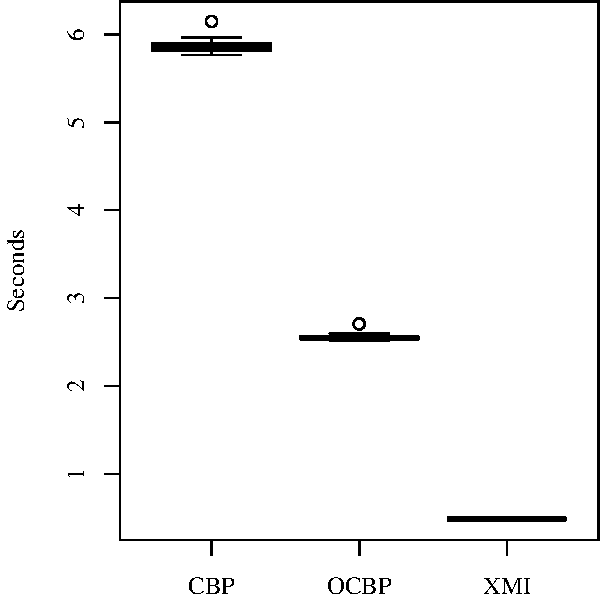
\includegraphics[width=\linewidth]{images/load_time_bpmn2}
        \caption{BPMN2}
        \label{fig:load_time_bpmn2}
    \end{subfigure}
    \hfill
    \begin{subfigure}{0.325\textwidth}
        \centering
        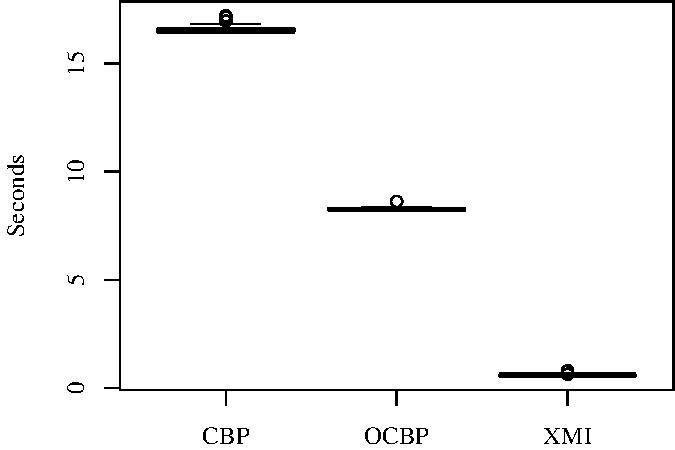
\includegraphics[width=\linewidth]{images/load_time_epsilon}
        \caption{Epsilon}
        \label{fig:load_time_epsilon}
    \end{subfigure}
    \hfill
    \begin{subfigure}{0.325\textwidth}
        \centering
        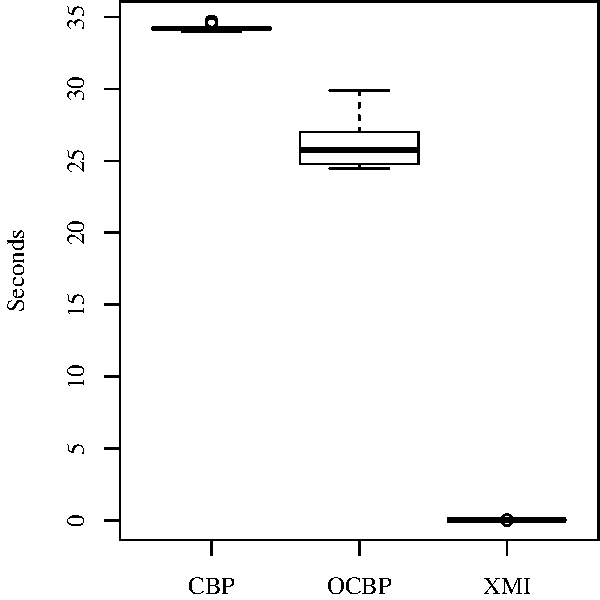
\includegraphics[width=\linewidth]{images/load_time_wikipedia}
        \caption{United States}
        \label{fig:load_time_wikipedia}
    \end{subfigure}
    \caption{Results for loading a model in original CBP (CBP), optimised CBP (OCBP), and for loading a state-based (XMI) representation.}
    \label{fig:loadtime}
\end{figure}

\subsection{Model Saving Time}
\label{subsec:saving_time_test}
 
 \vspace{-20pt}
  \begin{table}[ht]
     \small
     \centering
     \caption{The t-test results of saving time comparison between original CBP (CBP), optimised CBP (OCBP), and XMI.}
     \label{table:ttest_results_savetime}
     \begin{tabular}
         {|p{0.09\textwidth}|p{0.16\textwidth}|p{0.16\textwidth}|p{0.21\textwidth}|p{0.10\textwidth}|p{0.10\textwidth}|p{0.12\textwidth}|}
         \hline 
         
         % BPMN2 Save Time
         \textbf{Group} & \textbf{Mean} & \textbf{SD} & \textbf{Comparison} & \textbf{t}  & \textbf{df} & \textbf{p-value} \\  
         \hline 
         \multicolumn{7}{|c|}{BPMN2 Save Time} \\
         \hline 
         \textbf{CBP} & 0.0009671825    & 0.0012298125 & \textbf{CBP vs XM}I &  -175.58    & 22.011 & $<$ 2.2e-16 \\  
         \hline 
         \textbf{OCBP} & 0.0008048840   & 0.0001173053 & \textbf{CBP vs OCBP} & 0.6162 & 21.382  & 0.5443 \\  
         \hline 
         \textbf{XMI} & 0.3012216453   & 0.0079260992 & \textbf{OCBP vs XMI} & -177.76    & 21.009  & $<$ 2.2e-16 \\ 
         \hline 
         
         % EPSILON Save Time
         \multicolumn{7}{|c|}{Epsilon Save Time} \\
         \hline 
         \textbf{CBP} & 0.0006890233    & 0.0000335933 &  \textbf{CBP vs XM}I & -6.0088   &21.001 & $<$ 2.2e-16 \\
         \hline 
         \textbf{OCBP} & 0.0007997482   &  0.0000796359 & \textbf{CBP vs OCBP} & 160.06 & 28.244 & $<$ 1.7e-06 \\  
         \hline 
         \textbf{XMI} & 0.4002527172   & 0.005951101 & \textbf{OCBP vs XMI} & -314.8  & 21.008  & $<$ 2.2e-16 \\ 
         \hline 
         
         % WIKIPEDIA Save Time
         \multicolumn{7}{|c|}{United States Save Time} \\
         \hline 
         \textbf{CBP} & 0.0007063162     & 0.0000490199 & \textbf{CBP vs XM}I &  -46.192   & 21.078 & $<$ 2.2e-16 \\ 
         \hline 
         \textbf{OCBP} &0.0007538134   &  0.0000411298 & \textbf{CBP vs OCBP} &   -3.4816 & 40.77 & 0.001203 \\ 
         \hline 
         \textbf{XMI} &  0.0119452612   & 0.001140177 & \textbf{OCBP vs XMI} &  -46.009  & 21.055 & $<$ 2.2e-16 \\ 
         \hline
     \end{tabular}
     \justify
     $Mean$ = average, $SD$ = standard deviation, $t$ = t-test's $t$-$value$, $df$ = degree of freedom, $p$-$value$ = significance, the unit is seconds
 \end{table}
  
   This subsection presents the results of the saving time measurement of change-based models for each pair of the persistence types and cases and the t-test results of their comparisons (Table \ref{table:ttest_results_savetime} and Figure \ref{fig:savetime}). As discussed in\,\cite{yohannis2017turning}, CBP loading time penalties are balanced against the benefits that CBP brings, in terms of quicker, more precise differencing and more efficient incremental execution of model management programs.
    
    As shown in Table \ref{table:ttest_results_savetime} and Figure \ref{fig:savetime}, the performance of the two CBP implementations is not very different (all of the CBP vs OCBP comparisons' $p$-$values$ $>$ 2.2e-16, and for the BPMN2 case, the $p$-$value$ $>$ 0.1). This indicates that the cost of the extra work in the optimised CBP algorithm is negligible. On the other hand, both CBP implementations are significantly faster at saving changes than state-based XMI (The $means$ of both CBP implementations are smaller than XMI's $means$ and both CBP implementations have $p$-$values$ $<$ 2.2e-16 when compared to XMI). This is expected, as the CBP implementations only need append last change to the existing model file (their performance is thus relative to the number of changes since the last save), while the XMI implementation needs to reconstruct an XML document for the entire state of the model, and replaces the contents of the model file every time (and hence its performance is relative to the size of the entire model). 
    
     \begin{figure}[t]
        \begin{subfigure}{0.325\textwidth}
            \centering
            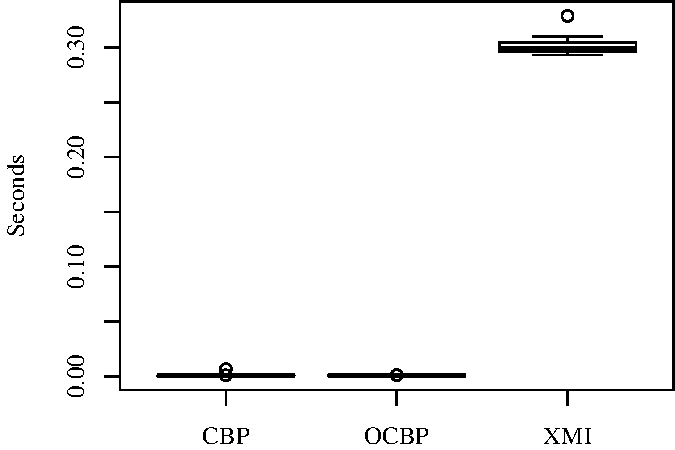
\includegraphics[width=\linewidth]{images/save_time_bpmn2}
            \caption{BPMN2}
            \label{fig:save_time_bpmn2}
        \end{subfigure}
        \hfill
        \begin{subfigure}{0.325\textwidth}
            \centering
            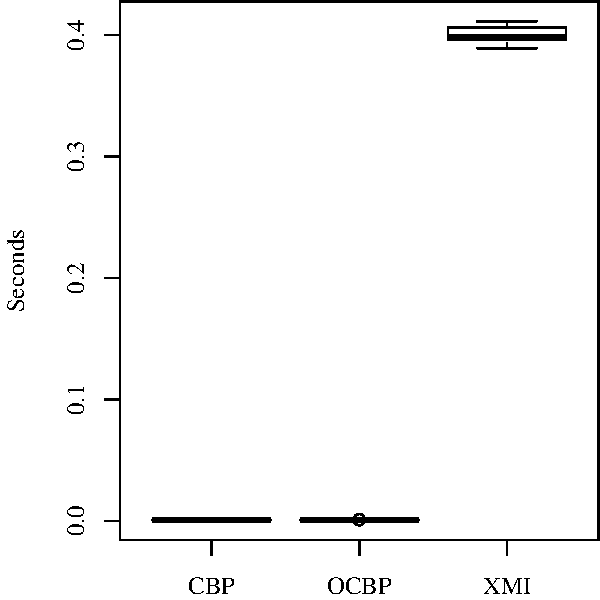
\includegraphics[width=\linewidth]{images/save_time_epsilon}
            \caption{Epsilon}
            \label{fig:save_time_epsilon}
        \end{subfigure}
        \hfill
        \begin{subfigure}{0.325\textwidth}
            \centering
            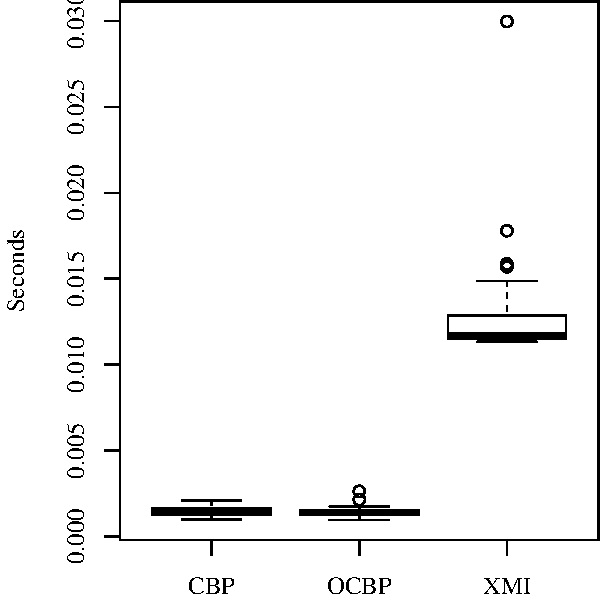
\includegraphics[width=\linewidth]{images/save_time_wikipedia}
            \caption{United States}
            \label{fig:save_time_wikipedia}
        \end{subfigure}
        \caption{A comparison on time required for persisting an event between original CBP (CBP), optimised CBP (OCBP), and XMI.}
        \label{fig:savetime}
    \end{figure}
    
    \vspace{-10pt}
    \subsection{Memory Footprint}
    \label{subsec:memory_consumption}
    
    \vspace{-20pt}
     \begin{figure}[ht]
        \begin{subfigure}{0.325\textwidth}
            \centering
            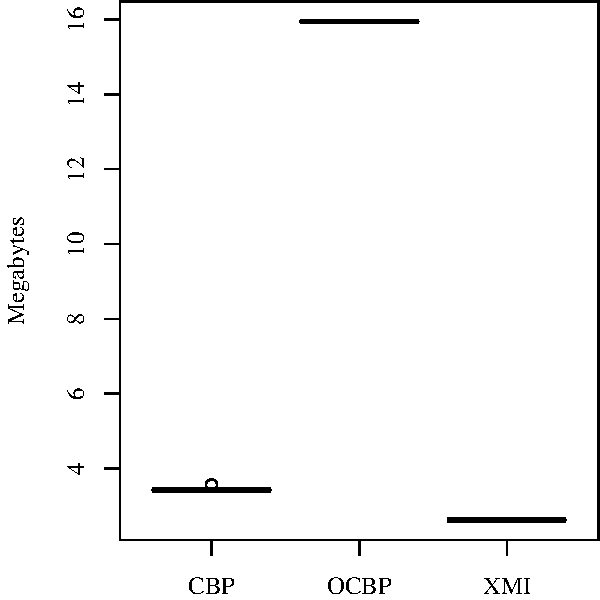
\includegraphics[width=\linewidth]{images/load_memory_bpmn2}
            \caption{BPMN2}
            \label{fig:load_memory_bpmn2}
        \end{subfigure}
        \hfill
        \begin{subfigure}{0.325\textwidth}
            \centering
            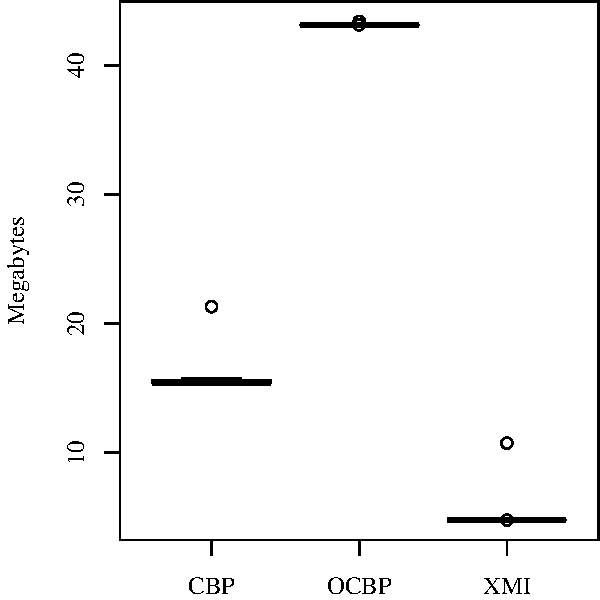
\includegraphics[width=\linewidth]{images/load_memory_epsilon}
            \caption{Epsilon}
            \label{fig:load_memory_epsilon}
        \end{subfigure}
        \hfill
        \begin{subfigure}{0.325\textwidth}
            \centering
            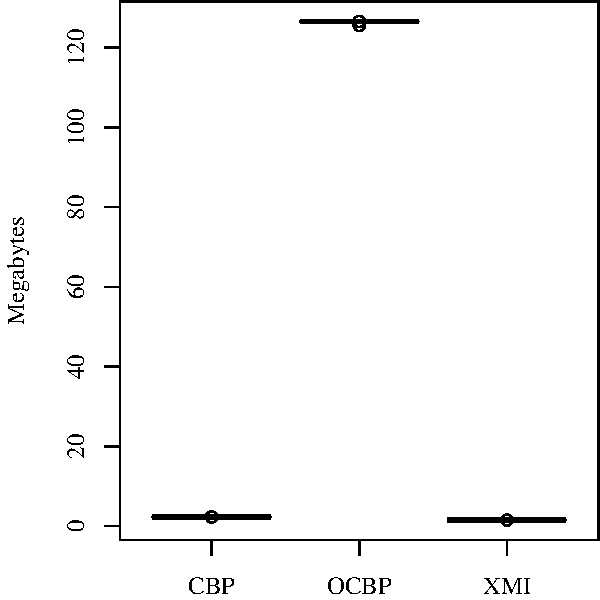
\includegraphics[width=\linewidth]{images/load_memory_wikipedia}
            \caption{United States}
            \label{fig:load_memory_wikipedia}
        \end{subfigure}
        \caption{A comparison on memory footprint after loading a model between original CBP (CBP), optimised CBP (OCBP), and XMI.}
        \label{fig:loadmemory}
    \end{figure}

     \begin{table}[t]
        \small
        \centering
        \caption{The t-test results of memory footprint comparison after loading a model between original CBP (CBP), optimised CBP (OCBP), and XMI.}
        \label{table:ttest_results_load_memory}
        \begin{tabular}
            {|p{0.09\textwidth}|p{0.16\textwidth}|p{0.16\textwidth}|p{0.21\textwidth}|p{0.10\textwidth}|p{0.10\textwidth}|p{0.12\textwidth}|}
            \hline 
            
            % BPMN2 Load Memory
            \textbf{Group} & \textbf{Mean} & \textbf{SD} & \textbf{Comparison} & \textbf{t}  & \textbf{df} & \textbf{p-value} \\  
            \hline 
            \multicolumn{7}{|c|}{BPMN2 Load Memory Footprint} \\
            \hline 
            \textbf{CBP} & 9.759984     & 0.0075976564 & \textbf{CBP vs XM}I &  4392.5   & 21.221 & $<$ 2.2e-16 \\  
            \hline 
            \textbf{OCBP} & 22.361524   & 0.0140733289 & \textbf{CBP vs OCBP} & -3695.7 & 32.283  & $<$ 2.2e-16 \\  
            \hline 
            \textbf{XMI} &  2.626207   & 0.0005516031 & \textbf{OCBP vs XMI} &  6572.4    & 21.065  & $<$ 2.2e-16 \\ 
            \hline 
            
            % EPSILON Load Memory
            \multicolumn{7}{|c|}{Epsilon Load Memory Footprint} \\
            \hline 
            \textbf{CBP} &15.741613    & 1.24805772 &  \textbf{CBP vs XM}I & 28.156   &  41.986 & $<$ 2.2e-16 \\
            \hline 
            \textbf{OCBP} & 43.148701   & 0.05587702 & \textbf{CBP vs OCBP} & -102.9 &21.084 & $<$ 2.2e-16 \\  
            \hline 
            \textbf{XMI} & 5.049445   & 1.27076960 & \textbf{OCBP vs XMI} & 140.49  & 21.081  & $<$ 2.2e-16 \\ 
            \hline 
            
            % WIKIPEDIA Load Memory
            \multicolumn{7}{|c|}{United States Load Memory Footprint} \\
            \hline 
            \textbf{CBP} & 2.289924     & 0.0002418689 & \textbf{CBP vs XM}I &   4523.5   & 25.161 & $<$ 2.2e-16 \\ 
            \hline 
            \textbf{OCBP} & 126.481274   & 0.2899075275 & \textbf{CBP vs OCBP} &   -2009.3 & 21 & $<$ 2.2e-16 \\ 
            \hline 
            \textbf{XMI} &  1.516487  & 0.0007646407 & \textbf{OCBP vs XMI} &  2021.8  & 21 & $<$ 2.2e-16 \\ 
            \hline
        \end{tabular}
        \justify
        $Mean$ = average, $SD$ = standard deviation, $t$ = t-test's $t$-$value$, $df$ = degree of freedom, $p$-$value$ = significance, the unit is megabytes
    \end{table}

    \vspace{-10pt}
    \begin{figure}
        \begin{subfigure}{0.325\textwidth}
            \centering
            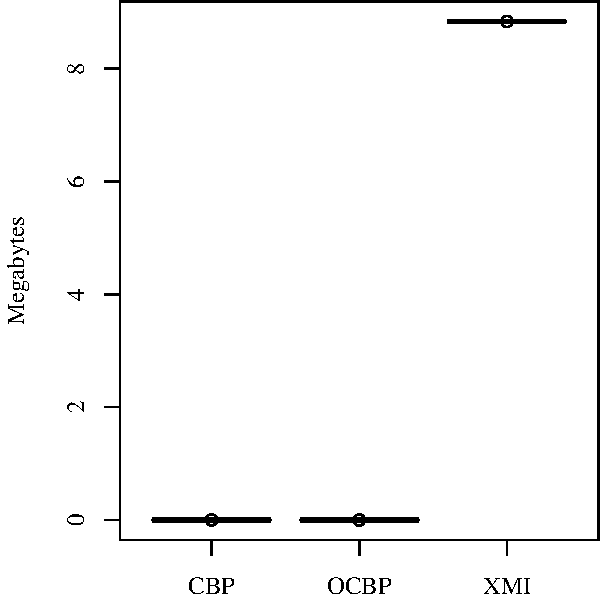
\includegraphics[width=\linewidth]{images/save_memory_bpmn2}
            \caption{BPMN2}
            \label{fig:save_memory_bpmn2}
        \end{subfigure}
        \hfill
        \begin{subfigure}{0.325\textwidth}
            \centering
            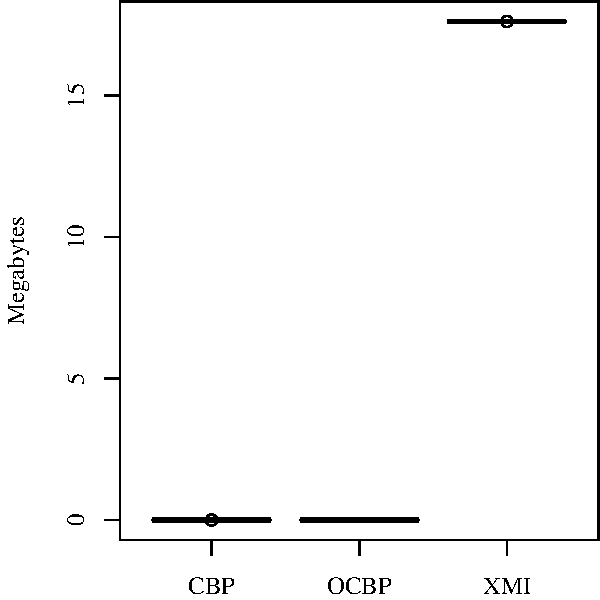
\includegraphics[width=\linewidth]{images/save_memory_epsilon}
            \caption{Epsilon}
            \label{fig:save_memory_epsilon}
        \end{subfigure}
        \hfill
        \begin{subfigure}{0.325\textwidth}
            \centering
            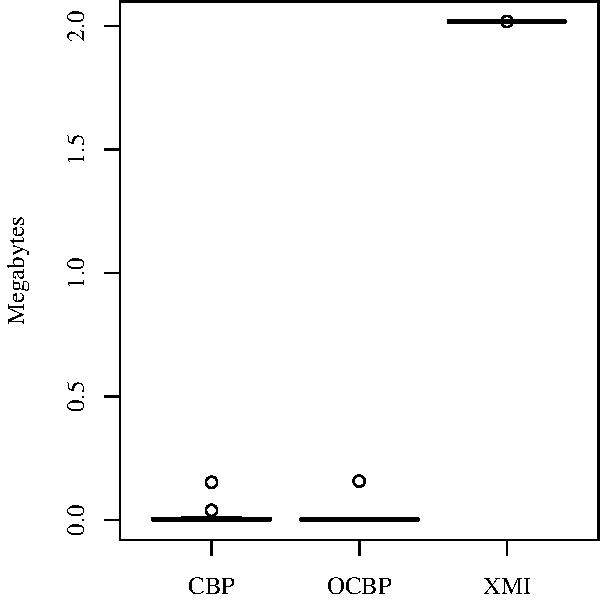
\includegraphics[width=\linewidth]{images/save_memory_wikipedia}
            \caption{United States}
            \label{fig:save_memory_wikipedia}
        \end{subfigure}
        \caption{A comparison on memory footprint after persisting an event between CBP, optimised CBP, and XMI.}
        \label{fig:savememory}
    \end{figure}

   \begin{table}[t]
       \small
       \centering
       \caption{The t-test results of memory footprint comparison after saving an event between original CBP (CBP), optimised CBP (OCBP), and XMI.}
       \label{table:ttest_results_save_memory}
       \begin{tabular}
           {|p{0.09\textwidth}|p{0.16\textwidth}|p{0.16\textwidth}|p{0.21\textwidth}|p{0.10\textwidth}|p{0.10\textwidth}|p{0.12\textwidth}|}
           \hline 
           
           % BPMN2 Save Memory
           \textbf{Group} & \textbf{Mean} & \textbf{SD} & \textbf{Comparison} & \textbf{t}  & \textbf{df} & \textbf{p-value} \\  
           \hline 
           \multicolumn{7}{|c|}{BPMN2 Save Memory Footprint} \\
           \hline 
           \textbf{CBP} &0.002348727    & 0.0000631206 & \textbf{CBP vs XM}I &  -489170    & 41.494 & $<$ 2.2e-16 \\  
           \hline 
           \textbf{OCBP} &0.002904364    & 0.000807634 & \textbf{CBP vs OCBP} & -3.2171 & 21.257 & 0.004091 \\  
           \hline 
           \textbf{XMI} & 8.836958545   & 0.0000564950 & \textbf{OCBP vs XMI} & -51180    &  21.206  & $<$ 2.2e-16 \\ 
           \hline 
           
           % EPSILON Save Memory
           \multicolumn{7}{|c|}{Epsilon Save Memory Footprint} \\
           \hline 
           \textbf{CBP} & 0.002498182    & 0.0000188317 &  \textbf{CBP vs XM}I & -4.3e+6   & 21.001 & $<$ 2.2e-16 \\
           \hline 
           \textbf{OCBP} & 0.003104000    &  0.000279853 & \textbf{CBP vs OCBP} & -10.131 & 21.19 & 1.405e-09 \\  
           \hline 
           \textbf{XMI} & 17.609975273   & 0.000002354 & \textbf{OCBP vs XMI} & -295090  &21.003  & $<$ 2.2e-16 \\ 
           \hline 
           
           % WIKIPEDIA Save Memory
           \multicolumn{7}{|c|}{United States Save Memory Footprint} \\
           \hline 
           \textbf{CBP} & 0.002503273  &0.0000186246 & \textbf{CBP vs XM}I &  -391970   & 40.522 & $<$ 2.2e-16 \\ 
           \hline 
           \textbf{OCBP} &  0.002817455   &  0.0008409904 & \textbf{CBP vs OCBP} &  -1.7518 & 21.021 &  0.09438 \\ 
           \hline 
           \textbf{XMI} &  2.019420727   & 0.0000153505 & \textbf{OCBP vs XMI} &  -11245  & 21.014 & $<$ 2.2e-16 \\ 
           \hline
       \end{tabular}
       \justify
       $Mean$ = average, $SD$ = standard deviation, $t$ = t-test's $t$-$value$, $df$ = degree of freedom, $p$-$value$ = significance, the unit is megabytes
   \end{table}

    Here we present the results of measuring the memory footprint after loading models (Table \ref{table:ttest_results_load_memory} and Figure \ref{fig:loadmemory}) and persisting single changes (Table \ref{table:ttest_results_save_memory} and Figure \ref{fig:savememory}) using the models from the three cases. The results show the significant memory overhead of the extra data structure when loading models (all the $means$ of optimised CBP are greater than all the $means$ of original CBP and all comparisons between both CBPs show $p$-$values$ $<$ 2.2e-16, Table \ref{table:ttest_results_load_memory}). Both CBPs are also outperformed by XMI in terms of memory footprint when loading models (all the $means$ of XMI are smaller than all the $means$ of both CBPs and all comparisons against XMIs show all $p$-$values$ $<$ 2.2e-16, Table \ref{table:ttest_results_load_memory}). In loading, XMI uses significantly less memory than the optimised CBP representation and performs slightly better than the original CBP.   
    
    \vspace{-10pt}
    In terms of saving, both CBP implementations persist a single change faster than XMI indicated by their $means$ that are smaller than the $means$ of XMI, and all the CBPs' t-tests with XMI show that their differences are significant at $p$-$value$ $<$ 2.2e-16 (Table \ref{table:ttest_results_save_memory}). The optimised CBP has more memory footprint against original CBP since the means of the optimised CBP for all cases are greater than the means of the original CBP. However, their memory footprints are not very different if we put 2.2e-16 as the p-value threshold. All their t-test results show $p$-$values$ $>$ 2.2e-16: the $p$-$values$ for BPMN2, Epsilon, and United States cases are 0.004091, 1.405e-9, and 0.09438 respectively.   
   
    \subsection{Threats to Validity and Limitations}
    \label{sec:limitations_and_future_work}
    In this work, we have only tested the algorithms on synthesised  models which may not be representative of the complexity and interconnectedness of models in other domains. Diverse characteristics of models in different domains can affect the effectiveness of the algorithm and therefore yield different outcomes. 
    
    So far, CBP optimisation only supports ordered and unique features. Support for duplicate values means that removal of an item does not necessarily result in the item not being present in the feature value. Additional information must be captured to persist the number of copies and positions of the feature members to properly generate the ignore list. 
    
    
    
   





    \section{Related Work}
    \label{sec:related_work}
    
    There are several non-XMI approaches to  state-based model persistence, using relational or NoSQL databases. For example, EMF Teneo\,\cite{eclipse2017teneo} persists EMF models in relational databases, while Morsa \cite{pagan2011morsa} and NeoEMF \cite{daniel2016neoemf} persist models in document and graph databases, respectively.  None of these approaches provides built-in support for versioning and models are eventually stored in binary files/folders which are known to be a poor fit for text-oriented version control systems like Git and SVN.
    
    Connected Data Objects (CDO) \cite{eclipse2017cdo}, provides support for database-backed model persistence as well as collaboration facilities, but its adoption necessitates the use of a separate version control system in the software development process (e.g. a Git repository for code and a CDO repository for models), which introduces fragmentation and administration challenges \cite{barmpis2014evaluation}. Similar challenges arise in relation to other model-specific version control systems such as EMFStore\,\cite{koegel2010emfstore}.
    
    
    
    \section{Conclusions and Future Work}
    \label{sec:conclusions}
    This paper proposes an efficient algorithm and supporting data structures for loading change-based models.  Performance is evaluated on synthesised models, with comparison against the existing change-based implementation, and state-based XMI. 
    Our results show considerable savings in terms of loading time with a negligible impact on saving time, but at the cost of a higher memory footprint.  In future, we intend to evaluate CBP against state-based persistence on real complex models.  We also plan to investigate the impact of change-based model persistence on the performance of change detection, model merging, and conflict resolution in the context of collaborative modelling.
    
    Meanwhile, the CBP approach can be further optimised, to consume less memory and to speed up parsing.  We are also exploring a hybrid persistence representation that offers a combination of state-based and change-based persistence. 
    
    \subsubsection*{Acknowledgments.} This work was partly supported by through a scholarship managed by \emph{Lembaga Pengelola Dana Pendidikan Indonesia} (Indonesia Endowment Fund for Education).
    %\clearpage
    \bibliography{references} 
    \bibliographystyle{splncs}
   
\end{document} 
